\subsection{Gtransfo\-Lin\-Rot  Class Reference}
\label{class_gtransfolinrot}\index{GtransfoLinRot@{Gtransfo\-Lin\-Rot}}
just here to provide a specialized constructor, and fit. 


{\tt \#include $<$gtransfo.h$>$}

Inheritance diagram for Gtransfo\-Lin\-Rot::\begin{figure}[H]
\begin{center}
\leavevmode
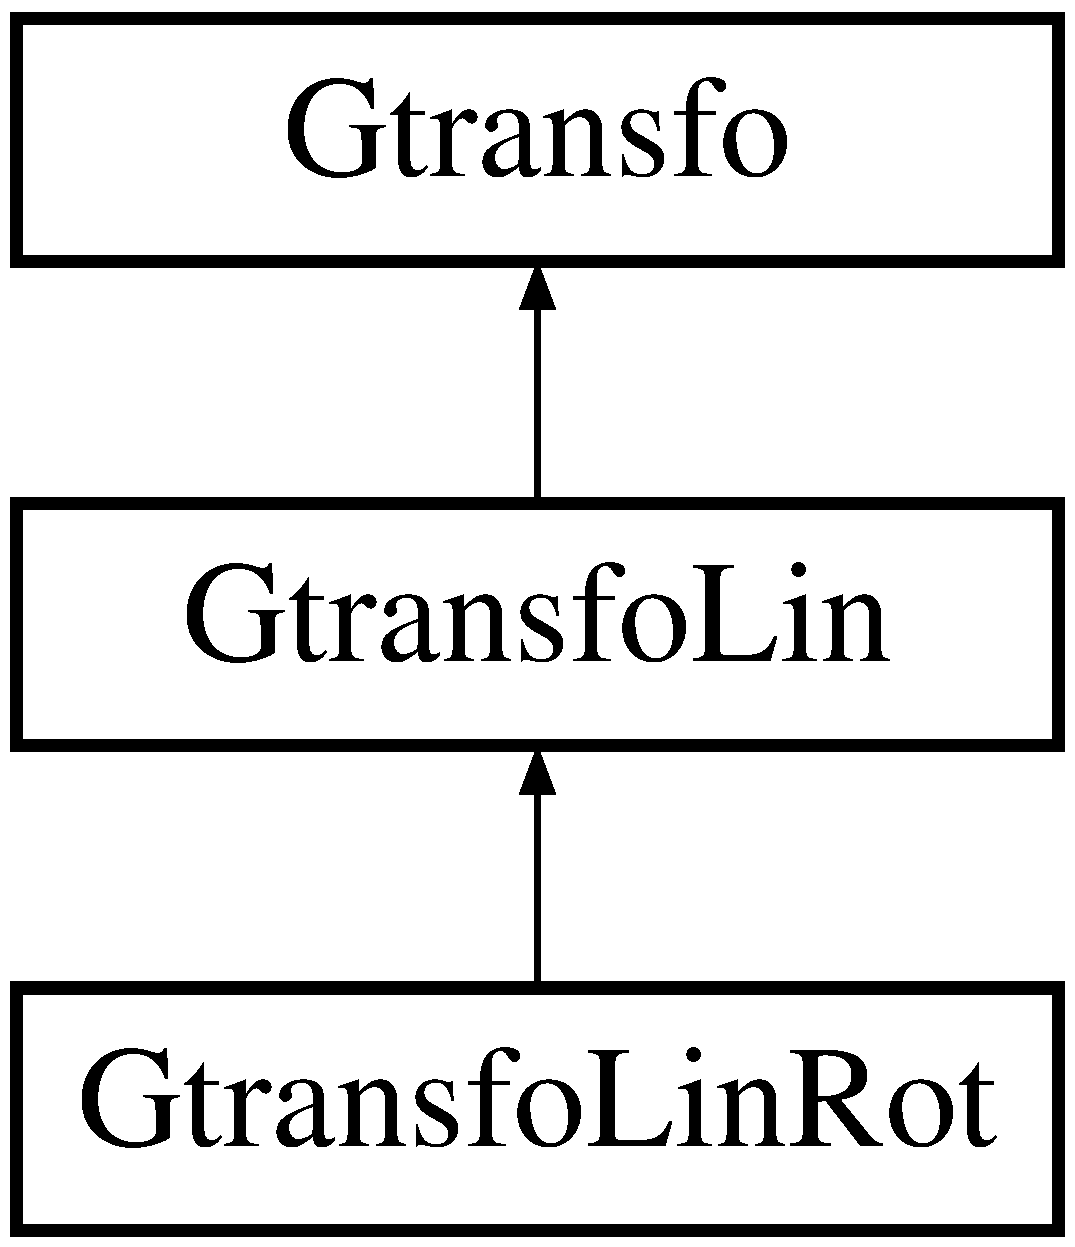
\includegraphics[height=3cm]{class_gtransfolinrot}
\end{center}
\end{figure}
\subsubsection*{Public Methods}
\begin{CompactItemize}
\item 
\index{GtransfoLinRot@{GtransfoLinRot}!GtransfoLinRot@{Gtransfo\-Lin\-Rot}}\index{GtransfoLinRot@{GtransfoLinRot}!GtransfoLinRot@{Gtransfo\-Lin\-Rot}}
{\bf Gtransfo\-Lin\-Rot} ()\label{class_gtransfolinrot_a0}

\item 
\index{GtransfoLinRot@{GtransfoLinRot}!GtransfoLinRot@{Gtransfo\-Lin\-Rot}}\index{GtransfoLinRot@{GtransfoLinRot}!GtransfoLinRot@{Gtransfo\-Lin\-Rot}}
{\bf Gtransfo\-Lin\-Rot} (const double Angle\-Rad, const {\bf Point} $\ast$Center=NULL, const double Scale\-Factor=1.0)\label{class_gtransfolinrot_a1}

\item 
double {\bf fit} (const Star\-Match\-List \&List, const {\bf Gtransfo} $\ast$Prior\-Transfo=NULL, const {\bf Gtransfo} $\ast$Posterior\-Transfo=NULL)
\begin{CompactList}\small\item\em fits a transfo to a list of star pairs (p1,p2).\item\end{CompactList}\item 
\index{Npar@{Npar}!GtransfoLinRot@{Gtransfo\-Lin\-Rot}}\index{GtransfoLinRot@{GtransfoLinRot}!Npar@{Npar}}
int {\bf Npar} () const\label{class_gtransfolinrot_a3}

\begin{CompactList}\small\item\em returns the number of parameters (to compute chi2's).\item\end{CompactList}\end{CompactItemize}


\subsubsection{Detailed Description}
just here to provide a specialized constructor, and fit.



\subsubsection{Member Function Documentation}
\index{GtransfoLinRot@{Gtransfo\-Lin\-Rot}!fit@{fit}}
\index{fit@{fit}!GtransfoLinRot@{Gtransfo\-Lin\-Rot}}
\paragraph{\setlength{\rightskip}{0pt plus 5cm}double Gtransfo\-Lin\-Rot::fit (const Star\-Match\-List \& {\em List}, const {\bf Gtransfo} $\ast$ {\em Prior\-Transfo} = NULL, const {\bf Gtransfo} $\ast$ {\em Posterior\-Transfo} = NULL)\hspace{0.3cm}{\tt  [virtual]}}\hfill\label{class_gtransfolinrot_a2}


fits a transfo to a list of star pairs (p1,p2).

After the fit this(Prior\-Transfo(p1)) yields approximately Posterior\-Transfo(p2). The returned value is the chi2. 

Reimplemented from {\bf Gtransfo\-Lin} {\rm (p.\,\pageref{class_gtransfolin_a9})}.

The documentation for this class was generated from the following file:\begin{CompactItemize}
\item 
{\bf gtransfo.h}\end{CompactItemize}
